\documentclass[12pt,a4paper]{article}

\usepackage[UTF8]{ctex}
\usepackage{amsmath,amssymb,bm}
\usepackage{graphicx}
\usepackage{booktabs}
\usepackage{longtable}
\usepackage{multirow}
\usepackage{hyperref}
\usepackage{cleveref}
\usepackage[backend=biber,style=gb7714-2015]{biblatex}
\addbibresource{refs.bib}

\title{LaTeX to Word Pipeline Test Document}
\author{Sample Project}
\date{\today}

\begin{document}

\maketitle
\tableofcontents

\section{引言}
本项目用于测试 \texttt{latex-to-word} 流水线是否能够正确处理：

\begin{itemize}
    \item 标题层级与目录；
    \item 图片与图题；
    \item 普通表格与长表格；
    \item 数学公式及其编号；
    \item 文献引用与文末参考文献；
    \item \verb|\ref|、\verb|\eqref|、\verb|\autoref|、\verb|\cref| 等交叉引用。
\end{itemize}

为了便于检查，本示例包含一个公式引用 \eqref{eq:state}、一个图片引用 \autoref{fig:sample-curve}、
以及一个表格引用 \cref{tab:params,tab:long}。


\section{实验结果}
本节给出一个测试图片。由\autoref{fig:sample-curve}可见，图像资源、图题与交叉引用应能被流水线识别。

\begin{figure}[htbp]
    \centering
    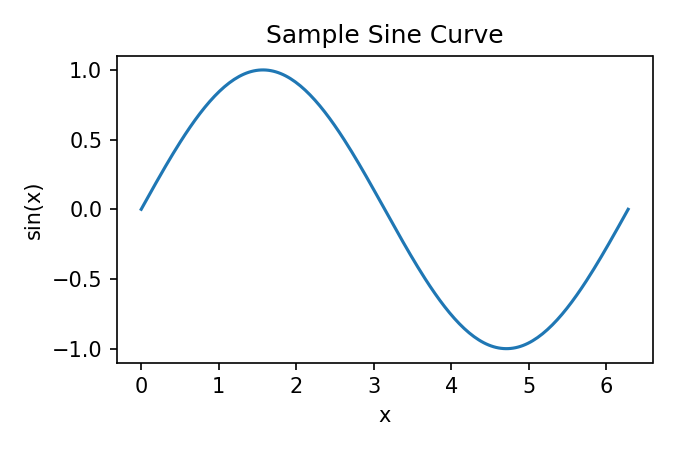
\includegraphics[width=0.72\linewidth]{figures/sample_plot}
    \caption{示例曲线图}
    \label{fig:sample-curve}
\end{figure}

\section{表格测试}
\cref{tab:params}给出了一个普通表格。\cref{tab:long}给出了一个较复杂的长表格，用于测试高风险对象识别。

\begin{table}[htbp]
    \centering
    \caption{示例参数表}
    \label{tab:params}
    \begin{tabular}{ccc}
        \toprule
        参数 & 符号 & 数值 \\
        \midrule
        采样周期 & $T_s$ & 0.01 s \\
        预测时域 & $N_p$ & 20 \\
        控制时域 & $N_c$ & 5 \\
        \bottomrule
    \end{tabular}
\end{table}

\begin{longtable}{cccc}
    \caption{示例长表格}\label{tab:long}\\
    \toprule
    序号 & 工况 & 指标 & 备注 \\
    \midrule
    \endfirsthead
    \toprule
    序号 & 工况 & 指标 & 备注 \\
    \midrule
    \endhead
    1 & 标准工况 & 0.95 & 基线 \\
    2 & 扰动工况 & 0.88 & 含外界扰动 \\
    3 & 约束工况 & 0.91 & 含输入饱和 \\
    4 & 参数摄动 & 0.86 & 含模型失配 \\
    \bottomrule
\end{longtable}

\section{公式测试}
下面给出一个带编号公式：
\begin{equation}
\label{eq:state}
\dot{\bm{x}}(t)=A\bm{x}(t)+B\bm{u}(t).
\end{equation}
其中，\eqref{eq:state}是最基本的状态方程。

再给出一个多行公式：
\begin{align}
J &= \int_{0}^{T}\left(\bm{x}^\mathsf{T}Q\bm{x}+\bm{u}^\mathsf{T}R\bm{u}\right)\,\mathrm{d}t, \\
\bm{u}^{\ast}(t) &= -R^{-1}B^\mathsf{T}P\bm{x}(t).
\end{align}

\section{参考文献测试}
这里给出两个文献引用：\cite{kalman1960new,bertsekas1995dynamic}。
如果转换顺利，文末参考文献应完整生成，且文内引用应保留可恢复结构。

\printbibliography

\end{document}
